\newpage
\chapter*{DAFTAR LAMPIRAN}
\addcontentsline{toc}{chapter}{DAFTAR LAMPIRAN}

\section*{Lampiran 1: Bukti Jawaban Responden (Mahasiswa UHN) terhadap Form}

\begin{figure}[H]
	\centering
	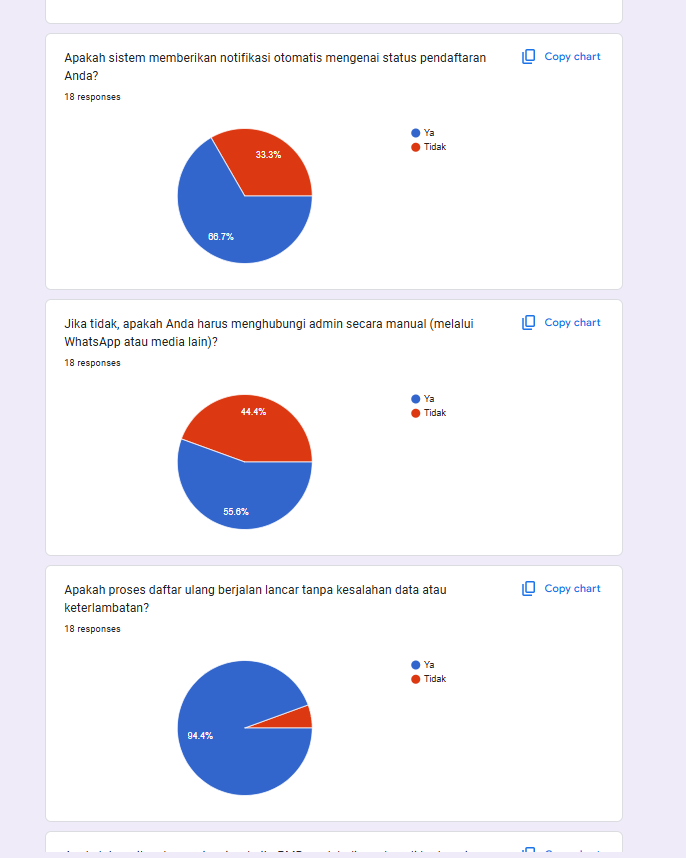
\includegraphics[width=0.85\textwidth]{figure/lampiran-responden.png}
	\caption*{Gambar D.1 Bukti Jawaban Responden}
\end{figure}

Bukti hasil jawaban pertanyaan responden form dari 18 mahasiswa baru di Universitas HKBP Nommensen. Dari \textit{responses} banyak yang merasa tidak ada kendala dalam melaksanakan PMB, namun ada juga yang mengalami keterlambatan dan harus menghubungi admin untuk meminta bantuan.\par

\section*{Lampiran 2: Bukti Wawancara dengan Pihak PSI UHN}

\begin{figure}[H]
	\centering
	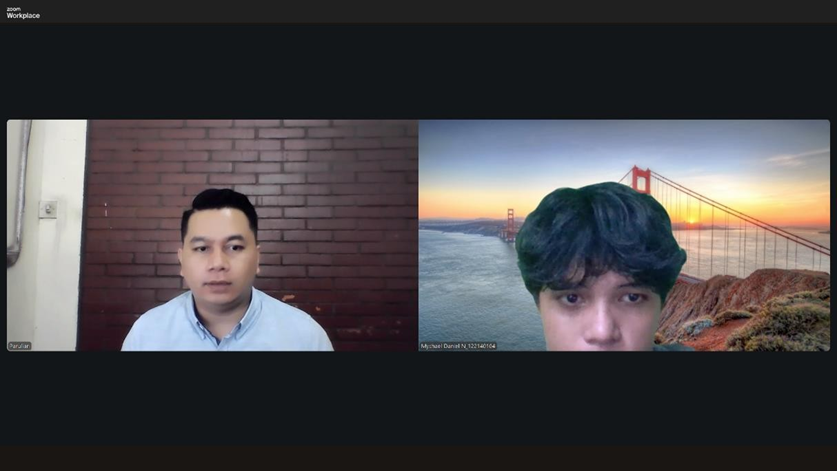
\includegraphics[width=0.85\textwidth]{figure/lampiran-wawancara.png}
	\caption*{Gambar D.2 Bukti Wawancara dengan Pihak PSI UHN}
\end{figure}

Bukti hasil wawancara dengan \textit{Network Administrator} Pusat Sistem Informasi, pengelola server Universitas HKBP Nommensen, Parulian Sirait, ST. Beliau merupakan penerima masukan dari keluhan PMB fakultas dan juga terlibat langsung dalam menghubungi camaba untuk proses daftar ulang dan verifikasi data.\par

\section*{Lampiran 3: Website PMB UHN}

\begin{figure}[H]
	\centering
	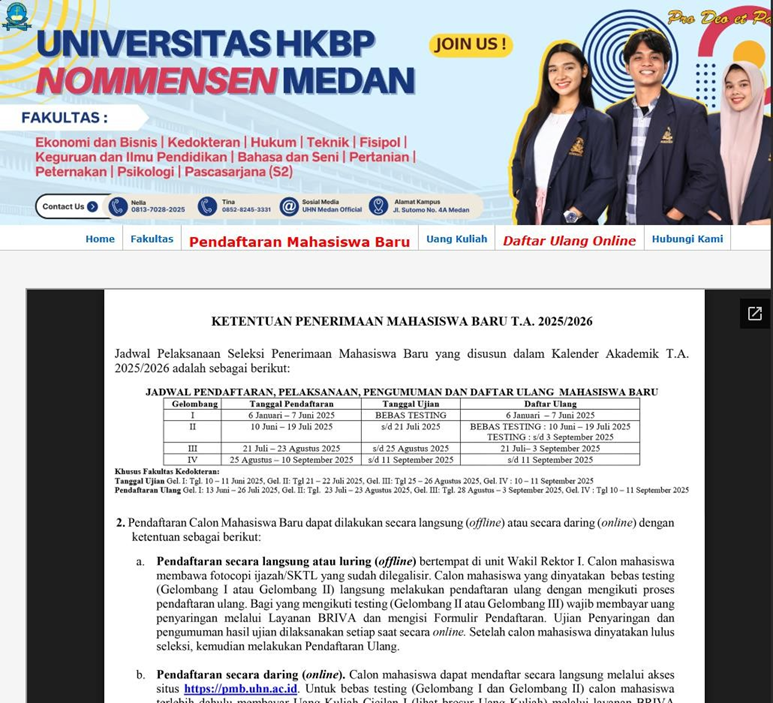
\includegraphics[width=0.85\textwidth]{figure/lampiran-website-pmb.png}
	\caption*{Gambar D.3 Tampilan PMB UHN}
\end{figure}

Tampilan halaman pendaftaran mahasiswa baru website PMB Universitas HKBP Nommensen.\par

\section*{Lampiran 4: Halaman Pendaftaran Ulang PMB}

\begin{figure}[H]
	\centering
	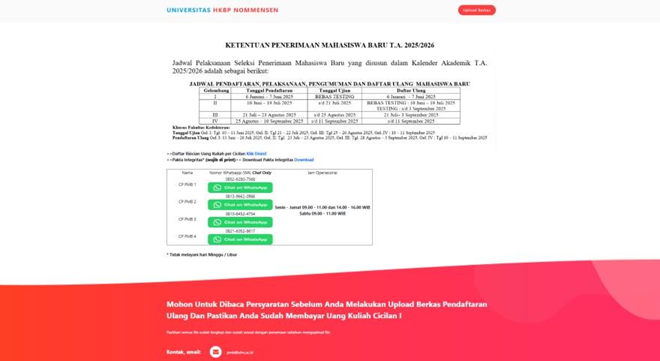
\includegraphics[width=0.85\textwidth]{figure/lampiran-daftar-ulang.png}
	\caption*{Gambar D.4 Tampilan Pendaftaran Ulang UHN}
\end{figure}

Tampilan halaman ketentuan website PMB Universitas HKBP Nommensen yang digunakan untuk mendaftar ulangkan para pendaftar.\par

\section*{Lampiran 5: Bukti Surat Balasan Permohonan Izin Penelitian Tugas Akhir}

\begin{figure}[H]
	\centering
	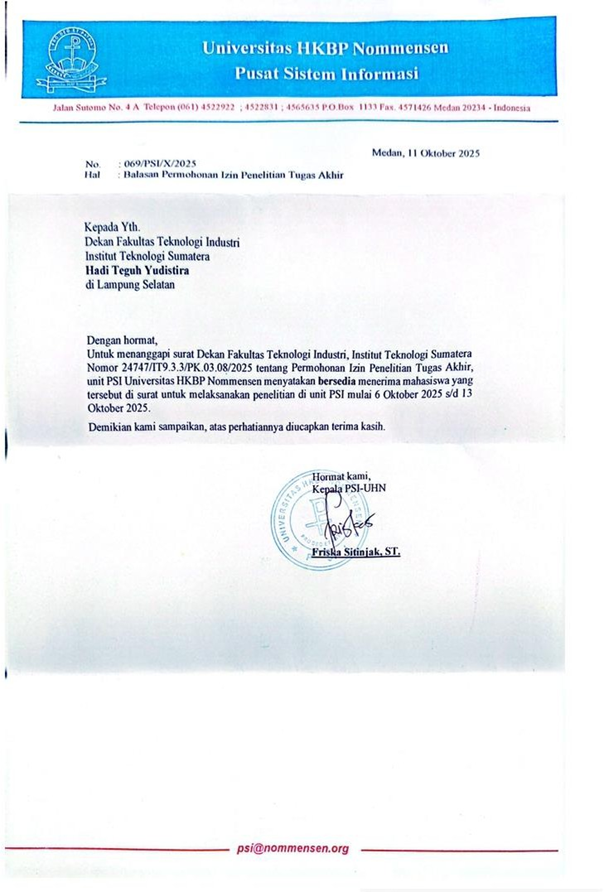
\includegraphics[width=0.7\textwidth]{figure/lampiran-surat-balasan.png}
	\caption*{Gambar D.5 Bukti Surat Balasan Permohonan Izin Penelitian}
\end{figure}

Bukti surat Balasan Permohonan Izin Penelitian Tugas Akhir yang sudah disetujui dan ditandatangani oleh pihak instansi Universitas HKBP Nommensen.\par

\section*{Lampiran 6: Bukti Surat Permohonan Izin Penelitian Tugas Akhir}

\begin{figure}[H]
	\centering
	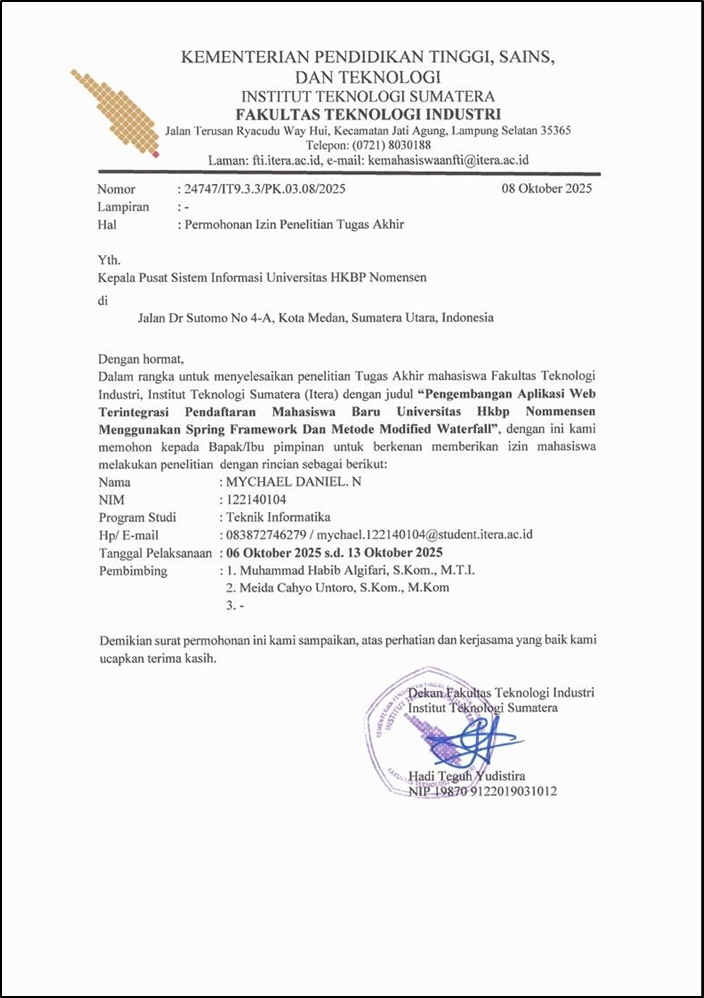
\includegraphics[width=0.7\textwidth]{figure/lampiran-surat-permohonan.png}
	\caption*{Gambar D.6 Tampilan Permohonan Izin Penelitian}
\end{figure}

Bukti surat Permohonan Izin Penelitian Tugas Akhir yang sudah disetujui dan ditandatangani oleh pihak Dekan Fakultas Teknologi Industri.\par

\section*{Lampiran 7: Surat Ketentuan Penerimaan Mahasiswa Baru}

\begin{figure}[H]
	\centering
	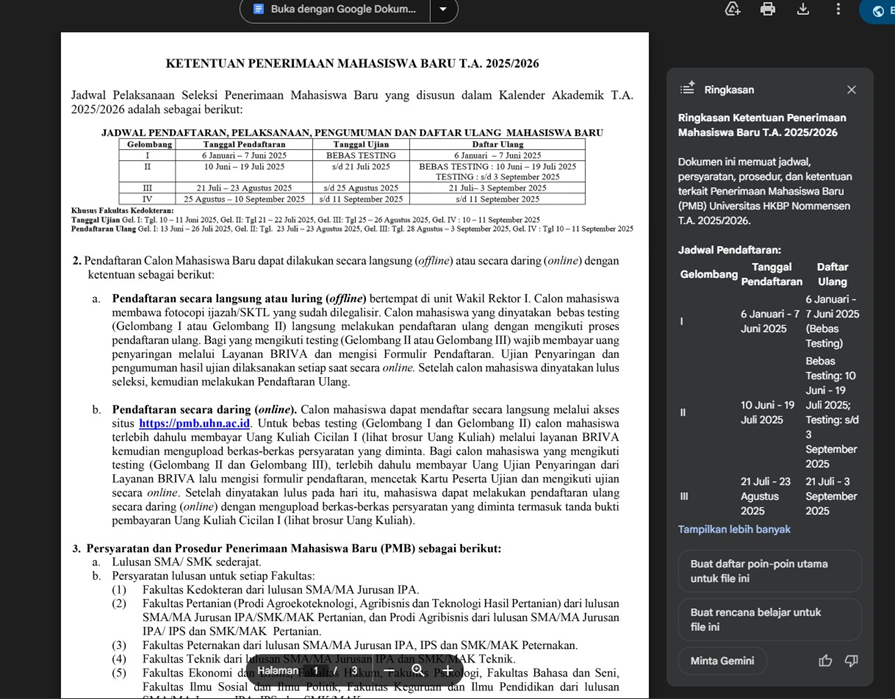
\includegraphics[width=0.7\textwidth]{figure/lampiran-ketentuan-pmb.png}
	\caption*{Gambar D.7 Ketentuan PMB Terbaru}
\end{figure}

Surat Ketentuan Penerimaan Mahasiswa Baru T.A. 2025/2026, yang berisikan ketentuan dan langkah-langkah calon mahasiswa baru untuk daftar menjadi mahasiswa Universitas HKBP Nommensen.\par

\section*{Lampiran 8: Data Pendaftar Ulang Calon Mahasiswa Baru UHN}

\begin{figure}[H]
	\centering
	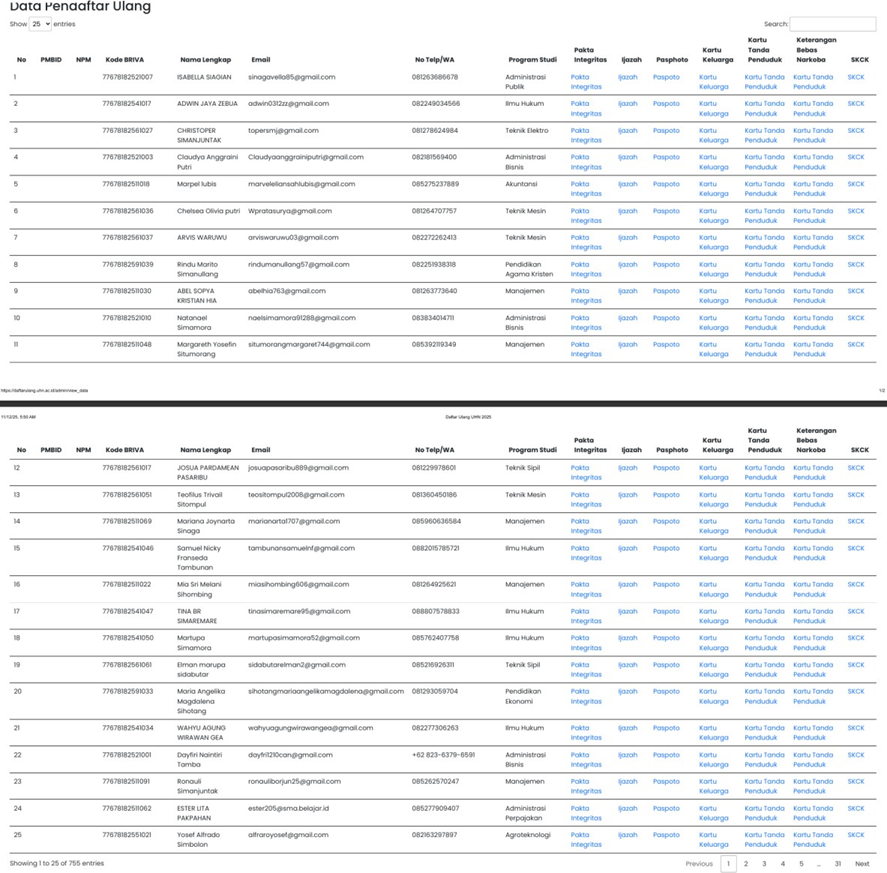
\includegraphics[width=0.85\textwidth]{figure/lampiran-data-pendaftar.png}
	\caption*{Gambar D.8 Data Pendaftar Ulang}
\end{figure}

Bukti daftar Data Pendaftar Ulang calon mahasiswa baru UHN, untuk Admin melihat jika camaba sudah membayar tagihan pendaftar secara manual.\par

\section*{Lampiran 9: SKPL PMB UHN}

\begin{figure}[H]
	\centering
	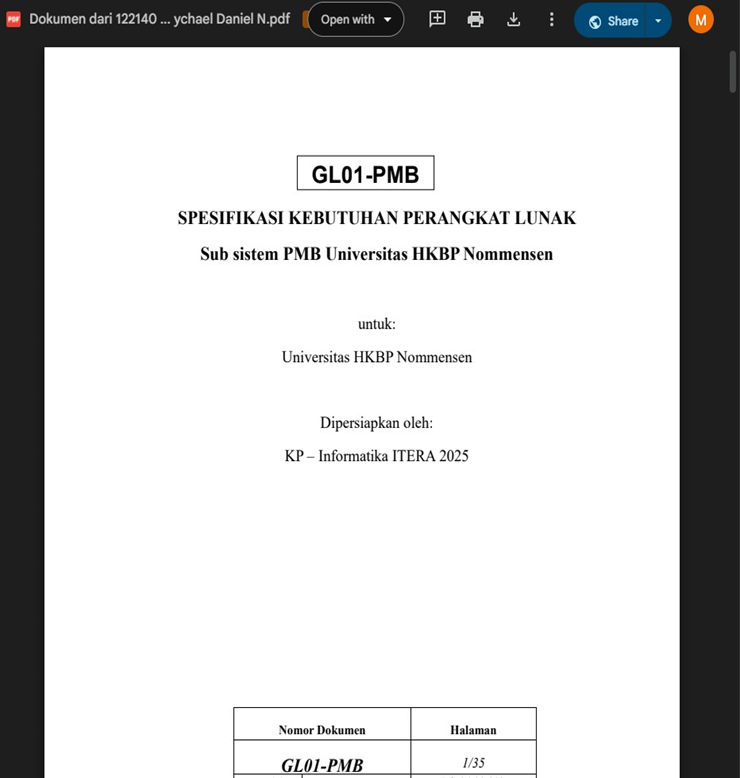
\includegraphics[width=0.85\textwidth]{figure/lampiran-skpl.png}
	\caption*{Gambar D.9 Lampiran SKPL}
\end{figure}

Bukti Lampiran Perancangan SKPL yang dibuat saat sedang melaksanakan PKL.\par
